% Step-by-step: from a pile of parts to a gantry the Kria can drive.
% Build with:  tectonic gantry-guide.tex
% Sizes come from dimensions.tex and robotics/cad/src/lib/dims.py.

\documentclass[10pt]{article}

\usepackage[margin=0.85in]{geometry}
\usepackage[T1]{fontenc}
\usepackage{lmodern}
\usepackage{microtype}
\usepackage{booktabs}
\usepackage{tabularx}
\usepackage{array}
\usepackage{enumitem}
\usepackage{xcolor}
\usepackage{graphicx}
\usepackage[hidelinks]{hyperref}
\usepackage{titlesec}
\usepackage{needspace}
\usepackage{listings}

\definecolor{accent}{HTML}{1F4E79}
\definecolor{muted}{HTML}{555555}
\definecolor{okgreen}{HTML}{2E7D32}
\definecolor{codebg}{HTML}{F4F6F8}
\titleformat{\section}{\needspace{12\baselineskip}\large\bfseries\color{accent}}{\thesection}{0.6em}{}
\titleformat{\subsection}{\needspace{8\baselineskip}\normalsize\bfseries}{\thesubsection}{0.6em}{}
\titlespacing*{\section}{0pt}{1.4em}{0.5em}
\titlespacing*{\subsection}{0pt}{1.0em}{0.3em}

\setlength{\parindent}{0pt}
\setlength{\parskip}{0.45em}
\setlist{nosep, leftmargin=1.6em}
\setlist[enumerate]{itemsep=0.25em}
\renewcommand{\arraystretch}{1.15}
\newcolumntype{L}{>{\raggedright\arraybackslash}X}

\newcommand{\mm}{\,mm}
\newcommand{\file}[1]{\texttt{#1}}
\newcommand{\gcode}[1]{\texttt{#1}}
\newcommand{\todo}[1]{\textcolor{red!70!black}{\textbf{Not designed yet:} #1}}
% A check you must pass before going on to the next step.
\newcommand{\gate}[1]{\par\smallskip\noindent\colorbox{okgreen!10}{\parbox{\dimexpr\linewidth-2\fboxsep}{\textcolor{okgreen}{\textbf{Check before moving on:}} #1}}\par\smallskip}
\newcommand{\warn}[1]{\par\smallskip\noindent\colorbox{red!8}{\parbox{\dimexpr\linewidth-2\fboxsep}{\textcolor{red!70!black}{\textbf{Careful:}} #1}}\par\smallskip}

\lstset{
  basicstyle=\ttfamily\small,
  backgroundcolor=\color{codebg},
  frame=none,
  columns=fullflexible,
  keepspaces=true,
  showstringspaces=false,
  xleftmargin=0.6em,
  framexleftmargin=0.6em,
  aboveskip=0.6em,
  belowskip=0.6em,
}

\title{\color{accent}\textbf{Chess robot: building the gantry, step by step}}
\author{Robotics subsystem, Tufts senior design}
\date{November 27, 2026}

\begin{document}
\maketitle
\vspace{-1.5em}

\begin{center}
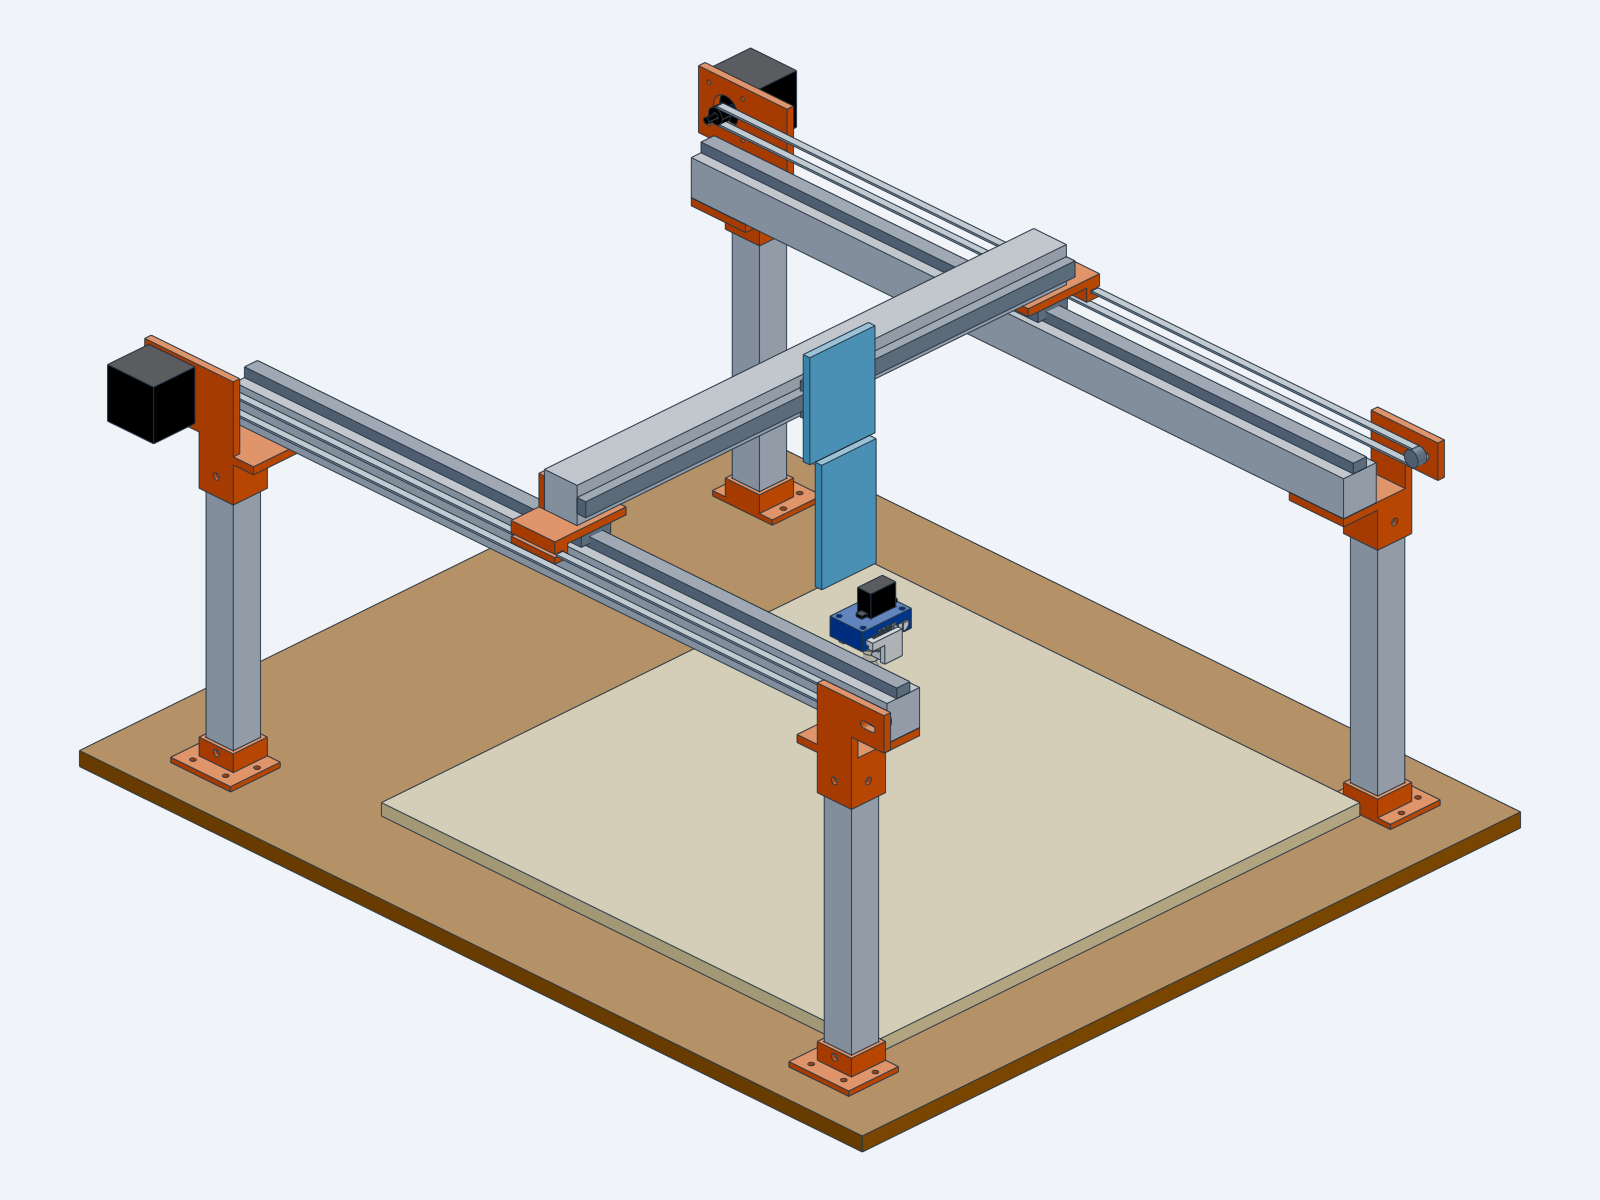
\includegraphics[width=0.72\textwidth]{images/gantry_frame.png}
\end{center}

This takes you from parts to a gantry the Kria can drive over USB. Do the steps in order. Each
section ends with a green check. Don't move on until it passes, because a problem found early
is a lot easier to fix than one found with everything bolted together.

The frame is the aluminum extrusion we already have: two 600\mm{} 3030 runways on four 2525
posts, and a 450\mm{} 3030 bridge that rolls along the runways on MGN12 linear rails. The motors
run off a BTT SKR Mini E3 V3 board with Marlin firmware, and the Kria sends it G-code over USB.
All the sizes are in \file{dimensions.pdf}, section 7.

\todo{the Y motor mount, the Y carriage with the Z axis, and the limit switch mounts. You can
do everything below for X now. Y and Z use the same steps once their parts exist.}

\setcounter{tocdepth}{1}
\tableofcontents

% ---------------------------------------------------------------------------
\section{Get everything together}

\textbf{Parts:} everything in the gantry and frame sections of \file{shopping-list.pdf}. The
important ones: 2 MGN12 rails of 600\mm{} with \textbf{MGN12C} (short) carriages, 1 MGN12 rail of
450\mm{} with an MGN12H carriage, 4 NEMA~17 motors, the SKR Mini E3 V3, a dual-motor splitter
cable, the 24\,V supply, GT2 belt, pulleys, idlers, limit switches, tee nuts and screws.

\textbf{Tools:} hex keys (2, 2.5, 3, 4, 5\mm), calipers, a square, a tape measure, a hacksaw and
miter box (or the makerspace chop saw), a file, zip ties, a multimeter, a soldering iron, needle-nose
pliers, and a laptop with a USB cable.

\section{Measure the extrusion}

The printed parts and the tee nuts assume these sizes. Check them now, before you print anything.

\begin{tabularx}{\textwidth}{l l L}
\toprule
Measure & Expected & If it's different \\
\midrule
3030 slot opening (the gap at the face) & 8\mm{} & Get tee nuts that fit. M6 tee nuts for 8\mm{} slots \\
2525 slot opening & 6\mm{} & Same. M5 tee nuts for 6\mm{} slots \\
3030 and 2525 outside size & 30.0 and 25.0 & Change \texttt{RUNWAY\_PROFILE} or \texttt{POST\_PROFILE} in \file{dims.py} and rebuild \\
\bottomrule
\end{tabularx}

\gate{the tee nuts you bought drop into the slots and slide along them.}

\section{Cut the posts}

\begin{enumerate}
  \item Mark all four 2525 bars at \textbf{231\mm}. Measure from a factory end, not a cut end.
  \item Cut in a miter box so the cut is square. Go slowly; aluminum clogs the blade if you push.
  \item File off the burrs, then stand all four on a flat table side by side.
\end{enumerate}

\gate{all four are within 0.5\mm{} of each other, and each stands upright on its cut end without
rocking. If one is long, file it down. Uneven posts make a twisted frame, and a twisted frame
makes the bridge bind.}

\section{Print the frame parts}

Every STL in \file{cad/STL/gantry/} is already laid in its print orientation, so just load it and
slice. Use the usual MK4 settings (0.15\mm{} QUALITY, PLA, no supports) but with \textbf{4 perimeters
and 40\% infill}, since these hold the frame up.

\begin{tabularx}{\textwidth}{c l L}
\toprule
Qty & File & What it is \\
\midrule
1 & \file{corner\_block\_motor\_plus\_y.stl} & $-X$ end of the $+Y$ runway, holds an X motor \\
1 & \file{corner\_block\_motor\_minus\_y.stl} & $-X$ end of the $-Y$ runway, holds the other X motor \\
1 & \file{corner\_block\_idler\_plus\_y.stl} & $+X$ end of the $+Y$ runway, holds a belt idler \\
1 & \file{corner\_block\_idler\_minus\_y.stl} & $+X$ end of the $-Y$ runway \\
1 & \file{bridge\_bracket\_plus\_y.stl} & Holds the $+Y$ end of the bridge and clamps that belt \\
1 & \file{bridge\_bracket\_minus\_y.stl} & Same for the $-Y$ end \\
4 & \file{post\_foot.stl} & Holds the bottom of each post \\
\bottomrule
\end{tabularx}

The \file{plus\_y} and \file{minus\_y} parts are mirror images. Label each one with a marker as it
comes off the printer so they don't get mixed up.

\gate{a 2525 post slides into a corner block's sleeve and a post foot's socket by hand, snug but
not forced. If it's too tight, raise \texttt{SLEEVE\_INNER} in \file{cad/src/lib/gantry.py} by
0.2 and reprint. Don't sand the sleeve; it'll end up loose on one side.}

% ---------------------------------------------------------------------------
\section{Build the frame}

Lay out the plywood base (about 720 $\times$ 605) with the 2$\times$2 tile or a 450\mm{} square
taped where the board goes. The $-X$ end is where the motors go, and the board isn't centered
on the base: there's more room past the $-X$ end for the motors.

\begin{enumerate}
  \item Slide each post into a foot. Put an M5 tee nut in the post's outside slot first, then
        an M5 $\times$ 10 through the foot into it. Snug, not tight.
  \item Push a corner block down onto the top of each post until the post bottoms out under the
        saddle. Add the two M5 screws and tee nuts (one through the outside face, one through the end).
  \item Drop two M6 tee nuts into the \textbf{bottom} slot of each runway, near each end. Rest the
        runway on the two corner blocks on its side and fasten it with M6 $\times$ 12 screws up through
        each saddle.
  \item Stand both runway assemblies on the base. Put the posts where \file{dimensions.pdf} says:
        runways 420\mm{} apart center to center (that's $y = \pm$210), posts 4.5\mm{} outside the board.
  \item Square the frame: measure the two diagonals between the outside corners of the
        runway tops. Nudge the feet until the diagonals match.
  \item Screw the feet to the base with four wood screws each, then tighten every screw on the frame.
\end{enumerate}

\gate{the diagonals match within 1\mm, the two runway tops are level with each other (put a
level across them on a straight board), and the runways are 420\mm{} apart at both ends.}

\section{Mount the rails}

\warn{never slide a carriage off the end of its rail. The balls fall out and it's ruined. Rails
come with a plastic stopper in the carriage; leave it in until the carriage is on the rail.}

\begin{enumerate}
  \item Drop M3 tee nuts into the \textbf{top} slot of each runway, one for every other hole
        in the rail (12 per runway).
  \item Lay a 600\mm{} rail on top of each runway, centered side to side, with its ends flush
        with the runway's ends. Put the MGN12\textbf{C} carriages on them.
  \item Fasten the rail with M3 $\times$ 10 screws, snug but not tight yet.
  \item Push the rail against a straight edge (another piece of extrusion clamped alongside works)
        and tighten from the middle out.
  \item Do the same for the 450\mm{} rail on the bridge's $+X$ face, centered top to bottom, with
        the MGN12H carriage. That's the face the claw will hang from.
\end{enumerate}

\gate{each carriage slides the whole length of its rail by hand, smoothly, with no tight spots.}

\section{Put the bridge on}

\begin{enumerate}
  \item Bolt a bridge bracket onto each X carriage with four M3 $\times$ 6 screws from the top. The
        counterbores let the heads sit flush. The bracket's cheek goes on the $-X$ side and its belt
        clamp sticks out past the runway, away from the board.
  \item Put two M6 tee nuts in the bridge's $-X$ slot near each end (the face without the rail).
  \item Set the bridge on the two brackets and fasten it through each cheek with M6 $\times$ 10
        screws. Snug only.
  \item Roll the bridge to the $-X$ end, then the $+X$ end, a few times, and \textbf{then} tighten
        the cheek screws. That lets the bridge settle square to the runways.
\end{enumerate}

\gate{you can push the bridge the full length of the runways with one finger on its center, and
it doesn't stick or twist anywhere. If it binds at one end, the runways aren't parallel there.
Loosen one rail, run the bridge back and forth, and tighten it again.}

% ---------------------------------------------------------------------------
\section{Mount the X motors and idlers (no belts yet)}

\begin{enumerate}
  \item Bolt an X motor to the outside of each motor corner block with four M3 $\times$ 10 screws.
        Its shaft goes through the plate toward the board.
  \item Slide a 20-tooth pulley onto each shaft, teeth toward the motor, and line its teeth up
        with the belt channel in the bridge bracket (about 11.5\mm{} from the motor face). Tighten
        one set screw onto the flat of the shaft, then the other.
  \item Put an M5 $\times$ 30 bolt through each idler block's slot from the outside, add washers as
        spacers, then the idler, then a nut. Use enough washers that the idler lines up with the
        pulley. Leave it loose for now.
\end{enumerate}

\gate{looking down the length of the runway, the pulley, the bracket's belt channel and the
idler are all in one straight line.}

% ---------------------------------------------------------------------------
\section{Wire the electronics}

\warn{the power supply's AC side is mains voltage. Have someone who has wired one before (a TA
or makerspace staff) check it before it's plugged in the first time: a fused, switched IEC inlet,
the earth wire on the supply's ground terminal, and the terminals covered. And never plug or
unplug a motor while the board has power. It can kill the driver.}

\begin{tabularx}{\textwidth}{l l L}
\toprule
What & Where on the SKR Mini E3 V3 & Notes \\
\midrule
24\,V supply & POWER IN (+ and $-$) & Through the emergency stop (see below) \\
Both X motors & X motor port, through the splitter & One motor is wired backwards. See below \\
Y motor & Y motor port & \\
Z motor & Z motor port & \\
X limit switch & X-STOP & At the $-X$ end, pressed by the bridge bracket \\
Y limit switch & Y-STOP & At the $-Y$ end of the bridge \\
Z limit switch & Z-STOP & At the \textbf{top} of Z travel, so homing lifts the claw first \\
Claw servo & PROBE / BLTouch header & Signal to the servo pin (PA1), plus 5\,V and ground \\
Laptop or Kria & USB-C & \\
\bottomrule
\end{tabularx}

\textbf{Emergency stop:} wire its normally-closed contacts in series with the 24\,V $+$ wire. Pressing
it cuts power to the motors and the board. Any time it's been pressed, home again (\gcode{G28})
before moving, because the board no longer knows where anything is.

\textbf{Limit switches:} wire each one's C and NC terminals to the two pins. Then the switch reads
``not pressed'' normally, and a broken wire looks the same as a pressed switch, which stops the
motor instead of crashing.

\textbf{Reversing one X motor:} the two X motors face opposite directions, so to push the bridge
the same way they have to turn opposite ways. On the 17HE15-1504S the wires are black A+, green
A$-$, red B+, blue B$-$ (check the datasheet that came with yours). On \textbf{one} X motor only, swap
black and green in its plug. Pop each pin out of the plastic housing by lifting its little tab
with a needle, swap them, and push them back in until they click.

\gate{with a multimeter, black to green on each motor reads a couple of ohms, and black to red
reads open. That proves the coils are paired right. Every switch reads closed when it's not pressed
and open when it is.}

% ---------------------------------------------------------------------------
\section{Flash Marlin}

The board comes with firmware for a 3D printer, which won't run without a heater. You'll build
Marlin with our settings once. It takes about 30 minutes the first time.

\begin{enumerate}
  \item Install VS Code. In its Extensions panel, install \textbf{PlatformIO IDE} and
        \textbf{Auto Build Marlin}.
  \item From \href{https://marlinfw.org/meta/download/}{marlinfw.org/meta/download}, download the
        latest \textbf{2.1.2.x} Marlin release and the \textbf{Configurations} release with the same
        number. Unzip both.
  \item In Configurations, find the folder \file{config/examples/Creality/Ender-3/BigTreeTech SKR Mini
        E3 3.0/} (search for ``SKR Mini E3 3.0'' if it has moved). Copy its \file{Configuration.h}
        and \file{Configuration\_adv.h} over the ones in \file{Marlin/} in the Marlin folder.
  \item Make the changes in the two tables below.
  \item Open the Marlin folder in VS Code, click the Auto Build Marlin icon on the left, and click
        \textbf{Build}. When it's done it shows where \file{firmware.bin} is.
  \item Copy \file{firmware.bin} onto a microSD card, put it in the board, and power it on.
        Wait a minute. When the file on the card has been renamed \file{FIRMWARE.CUR}, it worked.
\end{enumerate}

\needspace{16\baselineskip}
\textbf{Changes in \file{Configuration.h}} (search for each name with Ctrl+F):

\begin{tabularx}{\textwidth}{l l L}
\toprule
Setting & Change it to & Why \\
\midrule
\texttt{EXTRUDERS} & \texttt{0} & No extruder, so no heater checks \\
\texttt{TEMP\_SENSOR\_0}, \texttt{TEMP\_SENSOR\_BED} & \texttt{0} & No hot end or heated bed \\
\texttt{DEFAULT\_AXIS\_STEPS\_PER\_UNIT} & \texttt{\{ 80, 80, 400 \}} & GT2 on 20 teeth for X and Y, 8\mm{} lead screw for Z. Only 3 numbers now \\
\texttt{DEFAULT\_MAX\_FEEDRATE} & \texttt{\{ 200, 200, 20 \}} & mm/s \\
\texttt{DEFAULT\_MAX\_ACCELERATION} & \texttt{\{ 1000, 1000, 200 \}} & Gentle, so pieces don't swing \\
\texttt{X\_BED\_SIZE}, \texttt{Y\_BED\_SIZE} & \texttt{550}, \texttt{350} & The claw's reach in X and Y \\
\texttt{Z\_MAX\_POS} & \texttt{131} & Z travel \\
\texttt{Z\_HOME\_DIR} & \texttt{1} & Home Z upward, so the claw lifts before anything moves sideways \\
\texttt{NUM\_SERVOS} & \texttt{1} (uncomment it) & The claw servo, on pin PA1 \\
\texttt{BLTOUCH} & leave commented out & It would take over the servo pin \\
\texttt{FILAMENT\_RUNOUT\_SENSOR} & comment it out if it's on & \\
\bottomrule
\end{tabularx}

\textbf{Changes in \file{Configuration\_adv.h}:}

\begin{tabularx}{\textwidth}{l l L}
\toprule
Setting & Change it to & Why \\
\midrule
\texttt{X\_CURRENT} & \texttt{1200} & The two X motors share it, so each gets about 600\,mA. Plenty for this load \\
\texttt{Y\_CURRENT}, \texttt{Z\_CURRENT} & \texttt{800} & Quiet and cool. Raise it if a motor skips \\
\bottomrule
\end{tabularx}

If the build stops with an error, it names the setting it's unhappy with. With no extruder, errors
about a heater, PID, temperature, filament or the E axis usually just mean that \texttt{\#define} has to
be commented out too (put \texttt{//} in front of it). Then build again.

\gate{connect the laptop by USB and open \textbf{Pronterface} (from the Printrun project) at
115200 baud. Send \gcode{M115}. It answers with the Marlin version and today's build date.}

% ---------------------------------------------------------------------------
\section{First moves (still no belts)}

All of these are typed into Pronterface. Keep a hand near the emergency stop.

\begin{enumerate}
  \item \gcode{M119} lists every limit switch. All should say \texttt{open}. Press each switch by
        hand and send \gcode{M119} again; that one should say \texttt{TRIGGERED}. If it's backwards,
        it's wired to NO instead of NC.
  \item Stick a piece of tape on each X pulley like a flag. Send \gcode{G91} (relative moves) and then
        \gcode{M211 S0} (lets you move before homing), then \gcode{G1 X10 F600}.
  \item Watch the tops of both pulleys. Both should move toward $+X$ (the idler end). If both go
        toward $-X$, set \texttt{INVERT\_X\_DIR} the other way in \file{Configuration.h} and flash
        again. If they go \emph{opposite} ways, the reversed motor isn't reversed: recheck the
        black/green swap.
  \item Test homing with your finger as the switch: send \gcode{G28 X}. The pulleys turn toward
        $-X$. Press the X switch by hand and they should stop right away.
\end{enumerate}

\gate{both X pulleys turn the same way, toward $+X$ for a positive move, and homing stops the
instant the switch is pressed.}

\section{Put the X belts on}

\begin{enumerate}
  \item Cut two pieces of belt about \textbf{1400\mm} long.
  \item On each side: push one end through the bridge bracket's belt channel from the motor side,
        fold 30\mm{} back on itself teeth to teeth, and zip-tie the fold tight. The lump can't pull
        back through the channel.
  \item Run the belt around the motor pulley, back along the bottom, around the idler, and into the
        channel from the idler side. Pull it snug, fold and zip-tie that end too.
  \item Tension it by sliding the idler bolt outward in its slot, then tighten the nut. Press the
        middle of the lower run: it should give about 5\mm{} and twang like a low guitar string.
\end{enumerate}

\gate{both belts have about the same tension (same twang). Send \gcode{G1 X50 F1500} and back
with \gcode{G1 X-50 F1500}. The bridge moves smoothly and stays square: measure from the bridge to
the end of each runway; the two numbers should match within 1\mm.}

% ---------------------------------------------------------------------------
\section{Home and calibrate}

\begin{enumerate}
  \item Mount the X limit switch at the $-X$ end so the bridge bracket presses it about 5\mm{}
        before the carriage reaches the end of the rail.
  \item Send \gcode{M211 S1} to turn the soft limits back on, then \gcode{G28 X}. The bridge goes
        to $-X$, taps the switch, backs off and taps it again slowly.
  \item Check the distance: send \gcode{G90} then \gcode{G1 X0 F3000}, and put a pencil mark on
        the runway at the bracket's edge. Send \gcode{G1 X400}, mark again, and measure between
        the marks.
  \item If it isn't 400.0, fix the steps: new value $= 80 \times 400 \div$ what you measured.
        Send \gcode{M92 X}\textit{new value}, then \gcode{M500} to save it. Measure again.
\end{enumerate}

\gate{400\mm{} commanded is within 0.5\mm{} of 400 measured.}

\section{Repeatability: the real test}

Getting to the same spot every time matters more than any single number, because a piece placed
3\mm{} off is a piece that might not read.

\begin{enumerate}
  \item Put a strip of masking tape on the runway top, beside the rail, about 100\mm{} from the
        $-X$ end.
  \item Send \gcode{G28 X}, then \gcode{G1 X100 F6000}, and draw a sharp pencil line on the tape
        at the bridge bracket's edge.
  \item Go back and forth 20 times between \gcode{G1 X0} and \gcode{G1 X540}, then finish with
        \gcode{G1 X100}. Check the bracket edge against the line.
\end{enumerate}

\gate{after 20 round trips it's back within 0.5\mm{} of the mark. If it's drifting, a pulley set
screw is slipping (check it's on the shaft's flat) or a belt is loose.}

% ---------------------------------------------------------------------------
\section{Claw servo}

Do this \textbf{before} the pinion is on the servo, so a wrong angle can't break a jaw.

\begin{enumerate}
  \item Send \gcode{M280 P0 S90}. The servo goes to the middle of its range.
  \item Try \gcode{M280 P0 S70} and \gcode{M280 P0 S115}. The full jaw stroke takes about
        46\textdegree{} of servo turn, so ``closed'' and ``open'' will be roughly that far apart.
  \item Put the pinion on with the jaws closed and the servo at its closed angle. Find the open
        angle by stepping a few degrees at a time until the jaws are fully apart. Write both angles
        down; the Kria code needs them.
\end{enumerate}

\gate{the claw opens and closes on command and doesn't buzz when it's sitting still. If it buzzes
at the closed angle, back that angle off a couple of degrees. If the board resets every time the
servo moves, the servo is pulling too much current: power it from its own 5\,V supply and connect
that supply's ground to the board's ground.}

% ---------------------------------------------------------------------------
\section{Drive it from the Kria}

The board shows up on the Kria's Ubuntu as a serial port, usually \file{/dev/ttyACM0}
(\texttt{ls /dev/ttyACM*} to check). Install pyserial with \texttt{pip install pyserial}.

Marlin answers every line with \texttt{ok}. Always wait for the \texttt{ok} before sending the
next line. That's our acknowledgment that the move was accepted.

\begin{lstlisting}[language=Python]
import serial

class Gantry:
    def __init__(self, port="/dev/ttyACM0"):
        self.port = serial.Serial(port, 115200, timeout=30)
        self.port.reset_input_buffer()

    def send(self, line):
        """Send one line of G-code and wait for Marlin's ok."""
        self.port.write((line + "\n").encode())
        while True:
            reply = self.port.readline().decode(errors="replace").strip()
            if reply == "":
                raise TimeoutError(f"no answer to {line!r}")
            if reply.startswith("ok"):
                return
            if reply.startswith("Error") or "!!" in reply:
                raise RuntimeError(f"{line!r}: {reply}")
            # Anything else, like "echo:busy: processing", means keep waiting.

CLAW_OPEN, CLAW_CLOSED = 115, 70  # your angles from the servo step

gantry = Gantry()
gantry.send("G28")                    # home: Z up first, then X and Y
gantry.send("G90")                    # absolute coordinates
gantry.send("G1 X100 Y100 F6000")     # move over a square
gantry.send("M400")                   # wait until the move has really finished
gantry.send(f"M280 P0 S{CLAW_OPEN}")  # then open the claw
gantry.send("G4 P400")                # give the servo 0.4 s to get there
\end{lstlisting}

\textbf{Always send \gcode{M400} before \gcode{M280}.} Marlin says \texttt{ok} to a move as soon
as it's queued, not when it's finished. Without \gcode{M400} the claw would open while the gantry
is still moving.

\subsection{From squares to coordinates}

Marlin's coordinates start at the home position, not the board's center. Find the conversion once
by jogging, instead of trusting the numbers:

\begin{enumerate}
  \item Home, then jog the claw (Pronterface's arrows, or \gcode{G1}) until it's exactly over the
        center of a1. Write down X and Y from \gcode{M114}.
  \item Do the same for h8.
  \item Every other square is in between:
\end{enumerate}

\begin{lstlisting}[language=Python]
A1 = (100.0, 0.0)    # replace with your M114 reading over a1
H8 = (450.0, 350.0)  # and over h8

def square_xy(file, rank):
    """file and rank are 0 to 7 (a to h, 1 to 8)."""
    x = A1[0] + (H8[0] - A1[0]) * file / 7
    y = A1[1] + (H8[1] - A1[1]) * rank / 7
    return x, y
\end{lstlisting}

\gate{from the Kria, send the claw to all four corner squares and the center four, ten times
each in a random order. Every time, it's within 2\mm{} of the square's center.}

% ---------------------------------------------------------------------------
\section{If something's wrong}

\begin{tabularx}{\textwidth}{l L}
\toprule
What you see & Likely cause \\
\midrule
Motor buzzes but doesn't turn & One coil isn't connected. Check the plug and the pins you swapped \\
Moves the wrong way & Flip \texttt{INVERT\_X\_DIR} (or Y, Z) in \file{Configuration.h} and flash again \\
Bridge twists or binds while moving & One X motor isn't reversed, or the belts have different tension \\
Loses position over many moves & Set screw slipping, belt loose, or moving too fast. Lower the speed, then raise current by 100 \\
Motor or driver very hot & Current too high. Lower it by 100 and check again \\
Homing crashes into the end & Switch wired to NO, or \gcode{M119} shows it stuck \texttt{TRIGGERED} \\
\texttt{busy: processing} forever & A move is blocked. Hit the emergency stop, find what's in the way \\
Board resets when the servo moves & Servo needs its own 5\,V supply with a shared ground \\
Pronterface can't connect & Wrong port or baud rate (115200), or the Kria has the port open \\
\bottomrule
\end{tabularx}

\end{document}
